\chapter{Editor}

The editor provides methods to modify individual nodes and links and visualize data across the entire network. This chapter will explain the various options contained within the Editor and how to use them.

\begin{center}
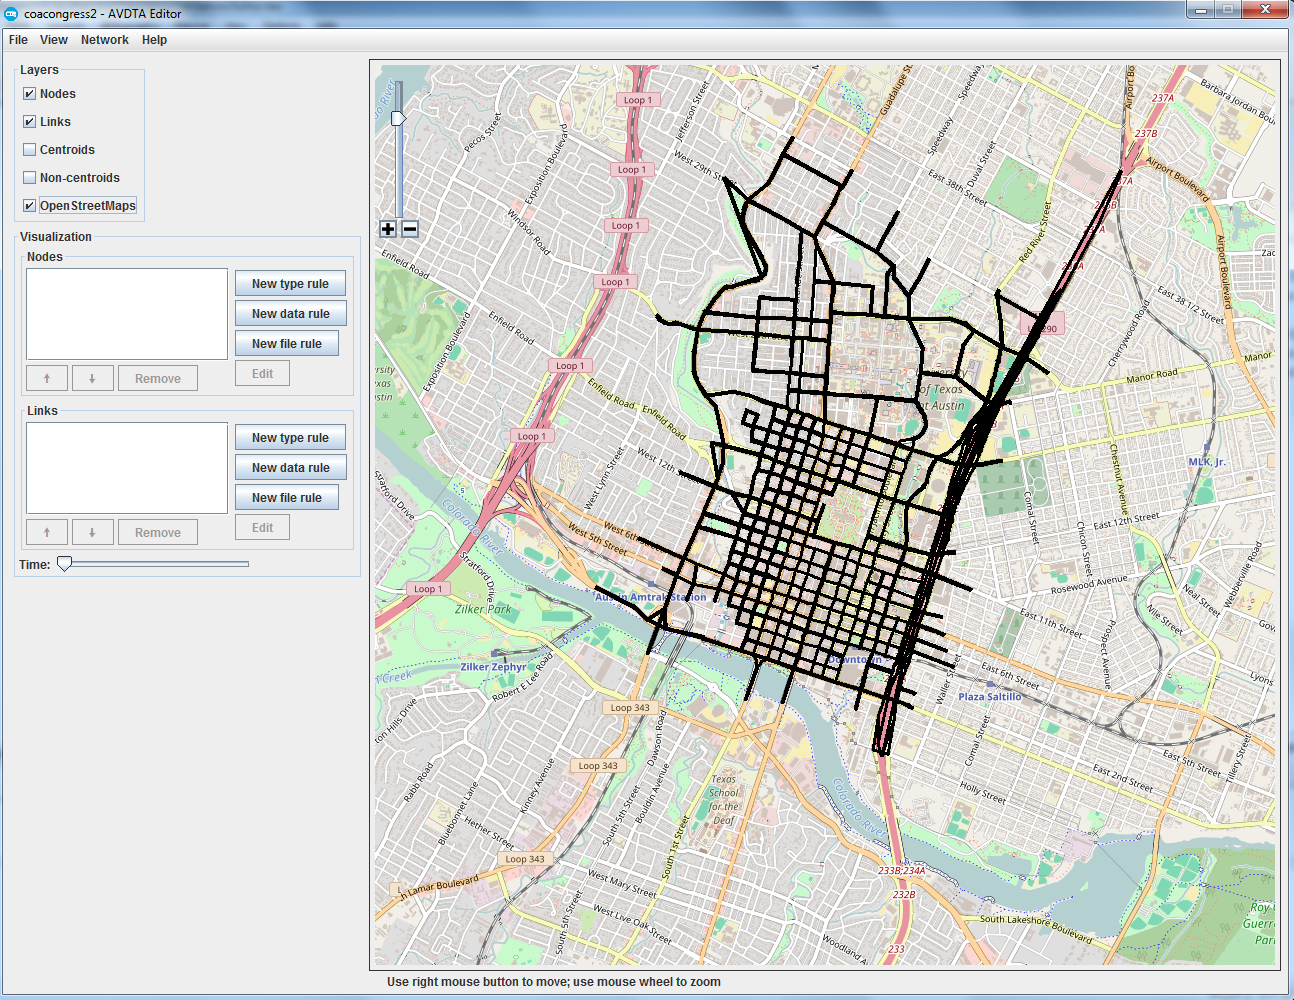
\includegraphics[width=\textwidth]{images/editor1.png}
\end{center}

\section{View options}


\subsection{Map}
The main feature of the visualization is an interactive map of the network. This map relies on the node and link coordinates in the \texttt{nodes.txt} and \texttt{link\_coordinates.txt} files to display properly. To move around the map, hold the right mouse button and drag the mouse. To zoom in or out, use the zoom slider, the mouse wheel, or the view menu options. 
%
There are also various selection modes (such as selected nodes or links) that may be used. Follow the instructions at the bottom of the map.

\begin{center}
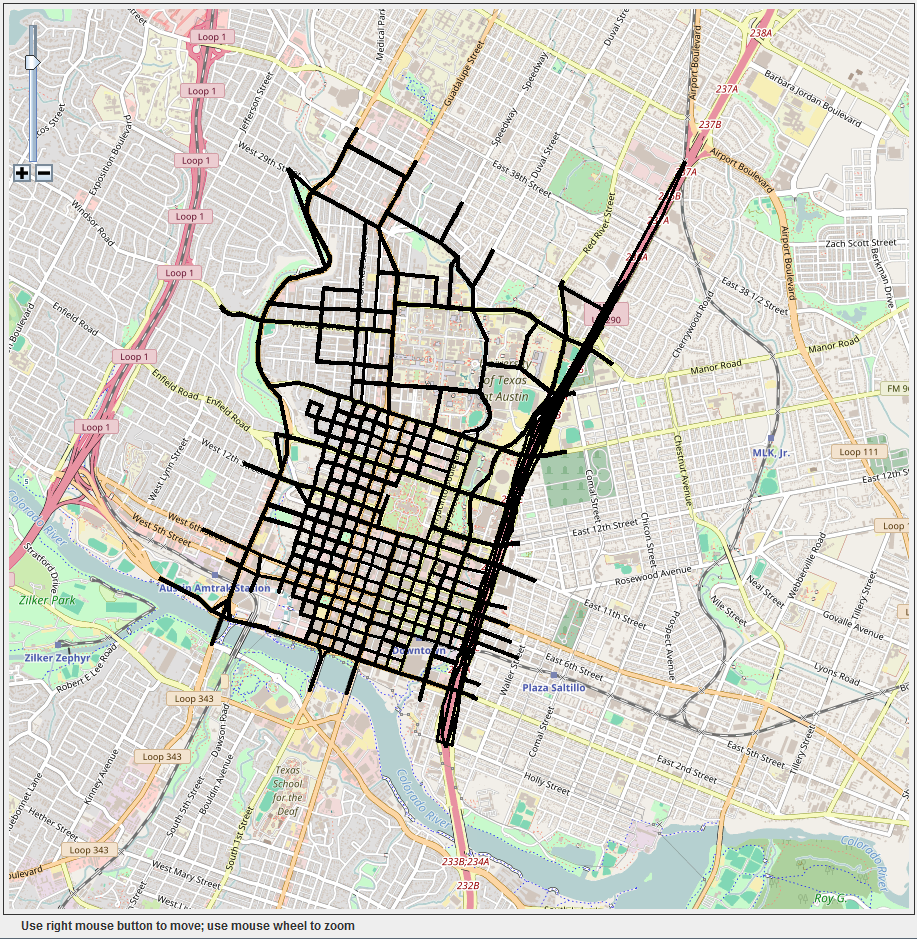
\includegraphics[width=0.6\textwidth]{images/editor4.png}
\end{center}

\subsection{View menu}
The view menu contains several options for controlling the view. The refresh button will repaint the view, and can be used if graphic glitches occur. Normally, though, the screen will automatically refresh as options are selected. The zoom in and out buttons provide an alternative way to control the zoom of the map.

The screenshot button will automatically take a screenshot of the current map display at its current resolution. (Note that the resolution used depends on the monitor resolution). User interface components such as the zoom slider will not appear in the screenshot, but any visualization applied will be captured.

The open and save visualization methods will open and save the \textit{visualization rules}. Section \ref{sec:visualization} discusses visualization rules in more detail. Note that the visualization rules are independent of the project, and can be opened and applied to any network. Of course, their effects will vary depending on the network.

\begin{center}
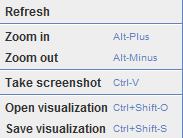
\includegraphics[scale=1]{images/editor3.png}
\end{center}

\subsection{Layers panel}

The layers menu controls which data is displayed on the map. The nodes and links checkboxes control whether nodes and links are displayed. Note that the default node display is only to display node ids. However, visualization rules may alter the way nodes are displayed.
%
The centroid and non-centroid checkboxes control whether centroids and centroid connectors, or intersections, are displayed. Normal links will be displayed regardless of whether these boxes are checked.
%
The OpenStreetMaps checkbox controls whether the OpenStreetMaps background is shown. 

\begin{center}
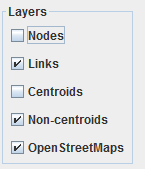
\includegraphics[scale=1]{images/editor2.png}
\end{center}

\section{Visualization panel}
\label{sec:visualization}

The visualization panel provides options for color-coding nodes and links in response to data (such as observed travel times), type (such as the intersection control), or via an external data source. There are two types of visualization rules: nodes and links. Rules are applied in the order shown, and it is possible to have multiple rules that could match a type of link. The time slider is used to control the input time for rules that might vary over time (such as observed travel times). If two links overlap, any links with a matching visualization rule will be displayed first.

\subsection{Node visualization}

There are three types of node visualizations: node type rule, node data rule, and node file rule. Click on the buttons to create new rules. There are also options to edit or remove existing rules and to change the order.

\subsubsection{Node type rule}

The node type rule matches nodes of a certain type, such as centroids, specific intersection controls, or specific policies for reservations. Use the comboboxes to select the type of nodes to match, and then select the color and radius to display matching nodes.
\begin{center}
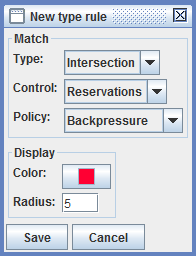
\includegraphics[scale=1]{images/editor6.png}
\end{center}

\subsubsection{Node data rule}

The data rule color-codes nodes on a scale between the minimum and maximum colors. The position on the scale for each node is determined by the data source and the minimum and maximum cutoff values. Nodes with a value less than the minimum use the minimum draw parameters; nodes with a value greater than the maximum use the maximum draw parameters. Hover over the data sources to obtain a description.

\begin{center}
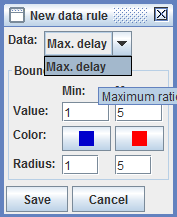
\includegraphics[scale=1]{images/editor6b.png}
\end{center}

\subsubsection{Node file rule}
The node file rule allows external visualization data to be applied. The input is a file with a specific format:
\begin{center}
\begin{tabular}{ccccc}
\hline
Node id & Radius & Red & Green & Blue\\\hline
\end{tabular}
\end{center}
\paragraph*{Node id}
the id of the node to be matched.

\paragraph*{Radius} the draw radius.

\paragraph*{Red, Green, Blue} Integers (between 0 and 255) that specify the color to draw the node.

\subsection{Link visualization}

There are three types of link visualizations: link type rule, link data rule, and link file rule. Click on the buttons to create new rules. There are also options to edit or remove existing rules and to change the order.

\subsubsection{Link type rule}

The node type rule matches links of a certain type, such as dynamic lane reversal, LTM, etc.. Use the comboboxe to select the type of links to match, and then select the color and width to display matching links.
\begin{center}
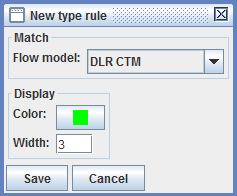
\includegraphics[scale=1]{images/editor6c.png}
\end{center}

\subsubsection{Link data rule}

The data rule color-codes nodes on a scale between the minimum and maximum colors. The position on the scale for each link is determined by the data source and the minimum and maximum cutoff values. Links with a value less than the minimum use the minimum draw parameters; links with a value greater than the maximum use the maximum draw parameters. Hover over the data sources to obtain a description.

\begin{center}
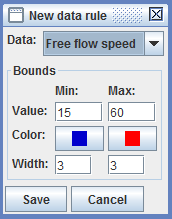
\includegraphics[scale=1]{images/editor6d.png}
\end{center}

\subsubsection{Link file rule}
The link file rule allows external visualization data to be applied. The input is a file with a specific format:
\begin{center}
\begin{tabular}{ccccc}
\hline
Link id & Width & Red & Green & Blue\\\hline
\end{tabular}
\end{center}
\paragraph*{Link id}
the id of the node to be matched.

\paragraph*{Width} the draw radius.

\paragraph*{Red, Green, Blue} Integers (between 0 and 255) that specify the color to draw the node.


\section{Network modification}
The editor also contains options to modify the network, found in the Network menu. Node and link options allow the modification of individual nodes and links, specifically.

\subsection{Node options}
Node options can be accessed from the Network menu and the Nodes submenu. 
\begin{center}
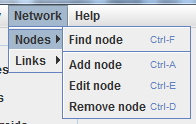
\includegraphics[scale=1]{images/editor7.png}
\end{center}

The find a node option allows you to enter a node id, and will center the map on the selected node. The add node option allows you to choose a location, then create a node at the selected location. The edit node option will allow you to click on an existing node and modify it. (If multiple nodes are selected, the editor will ask you to choose one). Both will bring up the edit node panel, which contains options to modify the node type, id, and location. When finished, click save.

\begin{center}
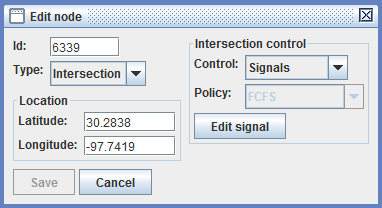
\includegraphics[scale=1]{images/editor7b.png}
\end{center}

Nodes with an intersection control that requires a signal also have the Edit Signal option. This opens the edit signal panel:
\begin{center}
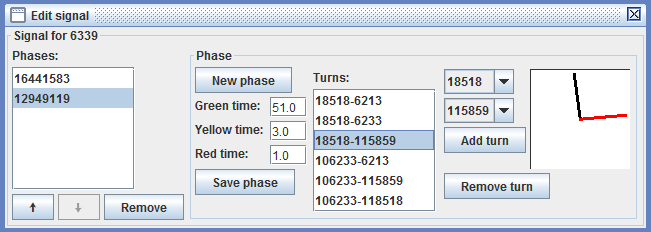
\includegraphics[scale=1]{images/editor7c.png}
\end{center}

The left side contains a list of phases, and options to remove or change the order of individual phases. Selecting a phase will allow it to be modified on the right side. This contains textfields to change the green time and clearance interval times, as well as a list of allowed turning movements. A turning movement consists of an incoming link and an outgoing link, and is displayed visually on the far right side. After editing a phase, click the save phase button to save it. The cycle will be saved automatically.

\subsection{Link options}

Link options can be accessed from the Network menu and the Links submenu.
\begin{center}
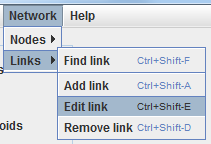
\includegraphics[scale=1]{images/editor8.png}
\end{center}

The find a link option allows you to enter a link id, and will center the map on the selected link. The add link option allows you to choose two nodes, then create a link connecting the two nodes. The edit link option will allow you to click on an existing link and modify it. When multiple links are selected, they will appear as separate tabs in the panel. 
Both will bring up the edit link panel, which contains options to modify the link flow model, id, and location. The location is a list of coordinates used for display purposes only. When finished, click save.
\begin{center}
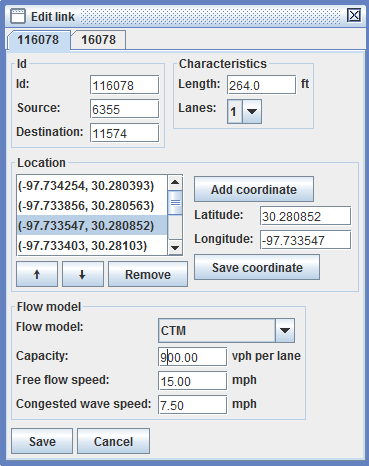
\includegraphics[scale=1]{images/editor8b.png}
\end{center}

%\section{Sanity check}

The editor contains a ``sanity check'' option under the Network menu. The sanity check scans through network and demand data, and attempts to report any errors discovered in an output file. The errors are color-coded to indicate their estimated severity. Although reported errors may not prevent solving the model, they are likely to introduce issues into the results. The paragraphs below describe the possible errors received, and the likely cause(s).

\subsection{Static OD file}

\paragraph*{\texttt{static\_od.txt} file is empty}
File is empty of entries as well as header data.

\paragraph*{Demand $x$ has non-positive id}
All entry ids must be positive.

\paragraph*{Duplicate OD id of $x$}
Each entry in the static OD file must have a separate id, and a duplicate id was found.

\paragraph*{OD $x$ type of $y$ not recognized}
The traveler or vehicle type for entry $x$ is not recognized (see Section \ref{sec:staticod}).

\paragraph*{Origin/destination $x$ does not appear in nodes}
Node $x$ does not have an entry in the \texttt{nodes.txt} file.

\paragraph*{Origin/destination $x$ is not a zone}
The type of node $x$ is not a zone, and traveler trips cannot depart or arrive at $x$. See Section \ref{sec:nodes}.

\paragraph*{OD $x$ has demand of $y$}
The demand $y$ is zero or negative for OD $x$.

\paragraph*{Malformed entry}
The entry (single line) is missing data or is in the wrong format.




\subsection{Dynamic OD file}

\paragraph*{\texttt{dynamic\_od.txt} file is empty}
File is empty of entries as well as header data.

\paragraph*{Demand $x$ has non-positive id}
All entry ids must be positive.

\paragraph*{Duplicate OD id of $x$}
Each entry in the static OD file must have a separate id, and a duplicate id was found.

\paragraph*{OD $x$ type of $y$ not recognized}
The traveler or vehicle type for entry $x$ is not recognized (see Section \ref{sec:staticod}).

\paragraph*{Origin/destination $x$ does not appear in nodes}
Node $x$ does not have an entry in the \texttt{nodes.txt} file.

\paragraph*{Origin/destination $x$ is not a zone}
Node $x$ is not a zone, and traveler trips cannot depart or arrive at $x$. See Section \ref{sec:nodes}.

\paragraph*{OD $x$ AST of $y$ not found in file \texttt{demand\_profile.txt}}
The AST $y$ does not appear in the \texttt{demand\_profile.txt} file.

\paragraph*{OD $x$ has demand of $y$}
The demand $y$ is zero or negative for OD $x$.

\paragraph*{Malformed entry}
The entry (single line) is missing data or is in the wrong format.